\section{Problem formulation}\label{sec:problem-formulation}
In this section we first describe the system model. Then, we present the optimization problem and prove its NP-hardness.
Final present an example problem to show the affect of the flexible resource allocation compared to fixed resource
allocation.

\begin{figure}[ht]
    \centering
    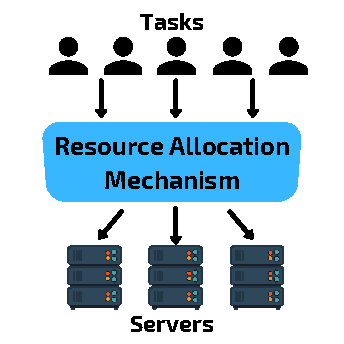
\includegraphics[width=0.6\linewidth]{figs/system_model.pdf}
    \caption{System Model}
    \label{fig:system_model}
\end{figure}

\subsection{System model}\label{subsec:system-model}
A sketch of the system is shown in Fig.~\ref{fig:system_model}.
We assume that in the system there is a set of servers $I = \{1,2,\ldots,\left|I\right|\}$ servers, which could be edge
clouds that can be accessed either through cellular base stations or WiFi access points (APs). These servers have
different types of limited resources: storage for the code/data needed to run a task (e.g., measured in GB),
computation capacity in terms of CPU cycles per time interval (e.g., measured in FLOP/s), and communication bandwidth
to receive the data and to send back the results of the task after execution (e.g., measured in Mbit/s). We assume
that the servers are heterogeneous in all their characteristics. More formally, we denote the storage capacity of
server $i$ with $S_i$, computation capacity with $W_i$, and the communication (bandwidth) capacity with $R_i$.

There is a set $J = \{1,2,\ldots,\left| J \right|\}$ of different tasks that require service from one of the servers.
\footnote{We focus on a single-shot setting in this paper. In practice, an allocation mechanism would repeat the
allocation decisions described here over regular time intervals, with longer-running tasks re-appearing on consecutive
time intervals. We leave a detailed study of this to future work.} Each task has a value, denoted $v_j$, representing
the value of running the task to its owner. To run any of these tasks on a server requires storing the appropriate
code/data on the same server. This storage size for the task $j$ is denoted as $s_j$ with the rate that the program
is transferred to the server as $s^{'}_j$. For a task to be computed successfully, it must fetch and execute
instructions on a CPU. We consider the total number of CPU cycles required for the program to be $w_j$, where the
number of CPU cycles are assigned to the task per unit of time as $w^{'}_j$. Finally, after the task is run and the
results obtained, the latter need to be sent back to the user. The size of the results for task $j$ is denoted with
$r_j$, and the bandwidth speed it is sent back to the user as $r^{'}_j$. Each task has a deadline, denoted by $d_j$,
as the maximum time for a task to be completed successfully. This time includes: the time required to send the
data/code to the server, run it on the server, and get back the results. We assume that there is an \emph{all} or
\emph{nothing} task execution reward scheme, meaning that the task value is awarded only if entire task loaded,
computed and the results sent back within the deadline.

\subsection{Optimization problem}\label{subsec:optimisation-problem}
Given the aforementioned assumptions from the system model, this requires two allocation mechanisms: the assignment of
tasks to servers and server resources to assigned task. This allocation mechanism is described by the following
optimisation where the variable $x_{i,j} \in \{0, 1\}$ describes if a task $j$ is running on server $i$.

\begin{align}
    \max & \sum_{\forall j \in J} v_j \left(\sum_{\forall i \in I} x_{i,j}\right)\label{eq:objective}\\
    \mbox{s.t.} \nonumber \\
    & \sum_{\forall j \in J} s_j x_{i,j} \leq S_i, &~ \forall i \in I,\label{eq:server_storage_constraint}\\
    & \sum_{\forall j \in J} w^{'}_j x_{i,j} \leq W_i, &~ \forall i \in I,\label{eq:server_computation_constraint}\\
    & \sum_{\forall j \in J} (r^{'}_j + s^{'}_j) \cdot x_{i,j} \leq R_i, &~ \forall i \in I,\label{eq:server_communication_constraint}\\
    & \frac{s_j}{s^{'}_j} + \frac{w_j}{w^{'}_j} + \frac{r_j}{r^{'}_j} \leq d_j, &~ \forall{j \in J},\label{eq:task_deadline}\\
    & 0 < s^{'}_j < \infty, &~ \forall{j \in J,}\label{eq:loading_speeds}\\
    & 0 < w^{'}_j < \infty, &~ \forall{j \in J,}\label{eq:compute_speeds}\\
    & 0 < r^{'}_j < \infty, &~ \forall{j \in J,}\label{eq:sending_speeds}\\
    & \sum_{\forall i \in I} x_{i,j} \leq 1, &~ \forall j \in J,\label{eq:server_task_allocation}\\
    & x_{i,j} \in \{0, 1\}, &~ \forall{i \in I},\forall{j \in J}.\label{eq:task_allocation}
\end{align}

The objective (Eq.\eqref{eq:objective}) is to maximize the total value over all tasks (i.e., the social welfare) that
are completed within the deadline (Eq.~\eqref{eq:task_deadline}. Constraints~\eqref{eq:server_storage_constraint},
~\eqref{eq:server_computation_constraint} and~\eqref{eq:server_communication_constraint} related to the finite resource
capacity of the servers, storage, computation and communication (bandwidth) respectively.
Constraint~\eqref{eq:server_storage_constraint} relates to the finite storage capacity for the task to store code/data
used to compute. With Eq.\eqref{eq:server_computation_constraint} being the finite computation capacity of each server.
The communication constraint (Eq.~\eqref{eq:server_communication_constraint}) comprises of two parts: the first for the
loading of the data/code onto the server, and the second for sending back the results to the user.
Constraint~\eqref{eq:task_deadline} forces the task to be completed within the task deadline, that being the sum of
time taken for all of the stages to complete in series (i.e.. loaded task onto server, computing the task, sending the
results back to the user). Note that if a task is not run on any server, this constraint can be satisfied by choosing
arbitrarily high bandwidth and CPU rates (as these resources do not use up any servers' resources in
Eq.~\eqref{eq:server_storage_constraint},~\eqref{eq:server_computation_constraint}
and~\eqref{eq:server_communication_constraint} when not allocated to server). The rates for each stage
($s^{'}_j$, $w^{'}_j$ and $r^{'}_j$) are all positive and finite (Eqs.~\eqref{eq:loading_speeds}
,~\eqref{eq:compute_speeds},~\eqref{eq:sending_speeds}). Further, every task is served by at most one server
(Eq.\eqref{eq:server_task_allocation}) as each task is either served or not by each server
(Eq.\eqref{eq:task_allocation}). \\


Using this optimisation problem, this is an extension of the knapsack problem that is well-studied and known to be
NP-hard with pseudo-polynomial time complexity using dynamic programming.
\begin{theorem}
    The optimisation problem as described in section~\ref{subsec:optimisation-problem} is NP-hard.
\end{theorem}
\begin{proof}
    The optimization problem without the constraint~\eqref{eq:task_deadline} is a 0--1 multidimensional knapsack
    problem~\cite{knapsackproblems_2004}, which is a generalization of a simple 0--1 knapsack problem. The latter is an
    NP-hard problem~\cite{knapsackproblems_2004}. Given this, it follows that the 0--1 multidimensional knapsack problem
    is also NP-hard. Since optimization problem (Eqs~\eqref{eq:objective} -~\eqref{eq:task_allocation}) is a
    generalization of a 0--1 multidimensional knapsack problem, it follows that it is NP-hard as well.
\end{proof}

\subsection{Example Problem Case}\label{subsec:example-problem-case}
Before we propose our novel allocation mechanisms for the allocation problem with elastic resources, we briefly
outline an example to illustrates why considering this elasticity is important. In this example, there are 12 potential
tasks and 3 servers (the exact settings can be found in table~\ref{table:example_tasks_properties} for the tasks and
table~\ref{table:example_servers_properties} for the servers). The figures~\ref{fig:fixed_resources_speeds}
and~\ref{fig:flexible_resources_speeds} represents each server as a group of three bars, each relating to the each
server's resource types, with the percentage of resources used by a task being the size of the bar.

\begin{figure}[th]
    \centering
    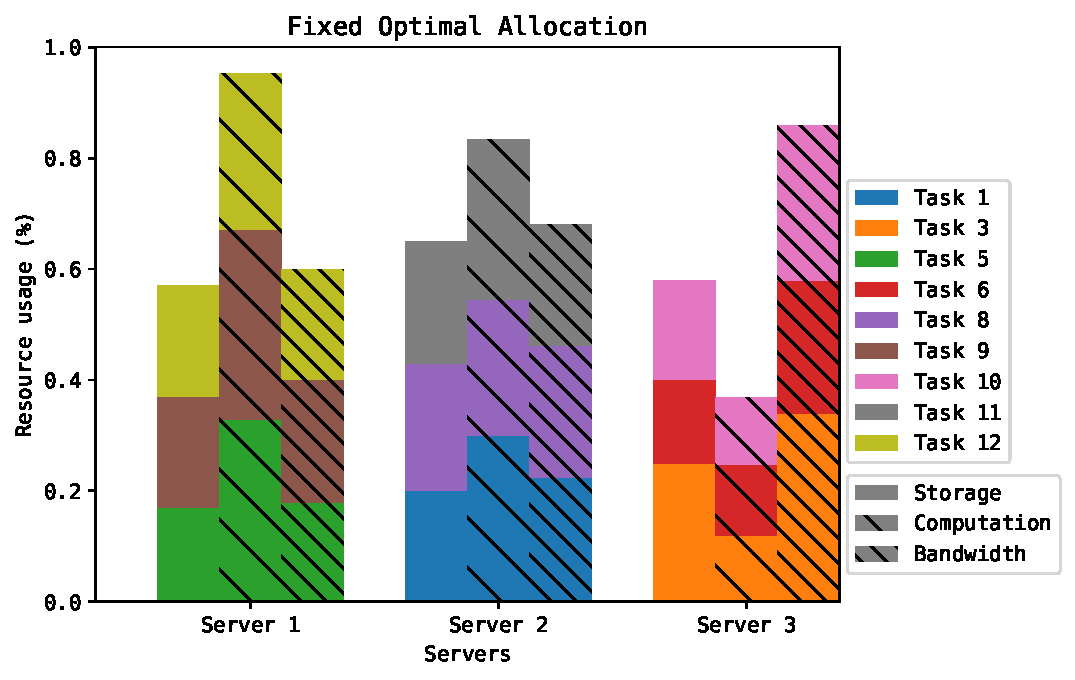
\includegraphics[width=\linewidth]{figs/allocation/fixed_optimal_allocation.pdf}
    \caption{Optimal solution with fixed resource speeds}
    \label{fig:fixed_resources_speeds}
\end{figure}

Figure~\ref{fig:fixed_resources_speeds} shows the best possible allocation if tasks have fixed resource speeds (that
were set by minimising the total amount of resources to be completed within the deadline). Here, only 9 of the tasks
are run, resulting in a total social welfare of 980 due to server 1 and 2's limited computational capacity and server
3' limited communication capacity.

\begin{figure}[th]
    \centering
    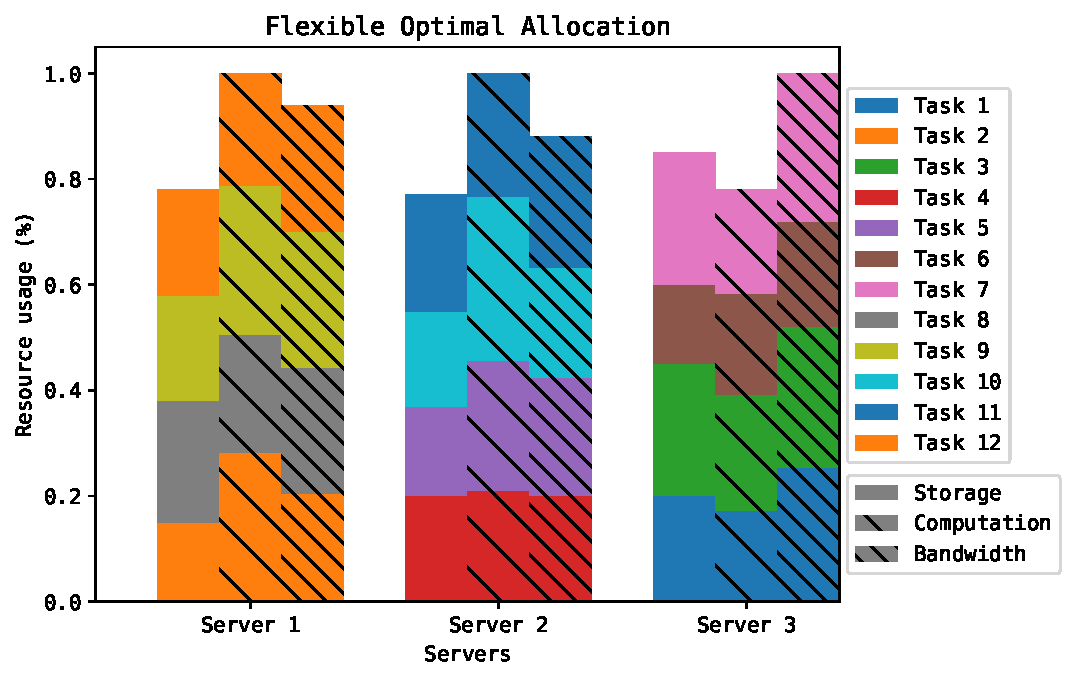
\includegraphics[width=\linewidth]{figs/allocation/flexible_optimal_allocation.pdf}
    \caption{Optimal solution with elastic resources. Compared to the fixed allocation, the elastic allocation is able
    to fully use all of its resources}
    \label{fig:flexible_resources_speeds}
\end{figure}

In contrast to figure~\ref{fig:fixed_resources_speeds}, Figure~\ref{fig:flexible_resources_speeds} depicts the optimal
allocation if elastic resources are considered. Here, all of the resources are used by the servers whereas the fixed
example~\ref{fig:fixed_resources_speeds} cant do this. In total, the elastic approach manages to schedule all 12 tasks
within the resource constraints, achieving a total social welfare of 1200 (an 18\% improvement over the fixed approach).

\begin{table}[h]
    \begin{tabular}{|c||c|c|c|}
        \hline
        Name & $S_i$ & $W_i$ & $R_i$ \\ [0.5ex] \hline\hline
        Server 1 & 400 & 100 & 220 \\ \hline
        Server 2 & 450 & 100 & 210 \\ \hline
        Server 3 & 375 & 90 & 250 \\ \hline
    \end{tabular}
    \caption{Table of server attributes}
    \label{table:example_servers_properties}
\end{table}

\begin{table}[h]
    \begin{tabular}{|c||c|c|c|c|c||c|c|c|}
        \hline
        Name & $v_j$ & $s_j$ & $w_j$ & $r_j$ & $d_j$ &  $s^{'}_j$ & $w^{'}_j$ & $r^{'}_j$ \\ [0.5ex] \hline\hline
        Task 1 & 100 & 100 & 100 & 50 & 10 & 30 & 27 & 17 \\ \hline
        Task 2 & 90 & 75 & 125 & 40 & 10 & 22 & 32 & 15 \\ \hline
        Task 3 & 110 & 125 & 110 & 45 & 10 & 34 & 30 & 17 \\ \hline
        Task 4 & 75 & 100 & 75 & 35 & 10 & 27 & 21 & 13 \\ \hline
        Task 5 & 125 & 85 & 90 & 55 & 10 & 24 & 28 & 17 \\ \hline
        Task 6 & 100 & 75 & 120 & 40 & 10 & 20 & 32 & 16 \\ \hline
        Task 7 & 80 & 125 & 100 & 50 & 10 & 31 & 30 & 19 \\ \hline
        Task 8 & 110 & 115 & 75 & 55 & 10 & 30 & 22 & 20 \\ \hline
        Task 9 & 120 & 100 & 110 & 60 & 10 & 27 & 29 & 24 \\ \hline
        Task 10 & 90 & 90 & 120 & 40 & 10 & 25 & 30 & 17 \\ \hline
        Task 11 & 100 & 110 & 90 & 45 & 10 & 30 & 26 & 16 \\ \hline
        Task 12 & 100 & 100 & 80 & 55 & 10 & 24 & 24 & 22 \\ \hline
    \end{tabular}
    \caption{Table of task attributes. The columns ($s^{'}_j$, $w^{'}_j$, $r^{'}_j$) are fixed speeds which are not
    considered by the flexible resource allocation.}
    \label{table:example_tasks_properties}
\end{table}